%%%%%%%%%%%%%%%%%%%%%%%%%%%%%%%%%%%%%%%%%%%%%%%%%%%%%%%%%%%%%%%%%%%%%%%%%%%%
%
%  Template code for the Undergraduate Research Scholars thesis program starting, updated by Undergraduate Research Scholars program staff. Version 6.0. Last Updated: Fall 2024
%  Modified by Tawfik Hussein from the template code for TAMU Theses and Dissertations starting Spring 2018, authored by Sean Zachary Roberson. Version 3.17.09.
%
%
%%%%%%%%%%%%%%%%%%%%%%%%%%%%%%%%%%%%%%%%%%%%%%%%%%%%%%%%%%%%%%%%%%%%%%%%%%%%%%%

%%%%%%%%%%%%%%%%%%%%%%%%%%%%%%%%%%%%%%%%%%%%%%%%%%%%%%%%%%%%%%%%%%%%%%%%%%%%%%%
%%%                           SECTION II: METHODS
%%%%%%%%%%%%%%%%%%%%%%%%%%%%%%%%%%%%%%%%%%%%%%%%%%%%%%%%%%%%%%%%%%%%%%%%%%%%%%%

%__________(0)_________
% Do not modify. This is the page heading

% THIS LINE PUTS "2. METHODS" AT THE TOP OF THE PAGE, BOLD-FACED AND 14-PT
\chapter{METHODS}


%__________(1)____________
% Modifications needed!

% THIS IS THE SECTION WHERE YOU TYPE IN THE TEXT RELATED TO YOUR METHODS. NOTICE THE DOUBLE \indent COMMAND THAT PROPERLY INDENTS THE BEGINNING OF EACH PARAGRAPH

\begin{figure}[H]
\centering
  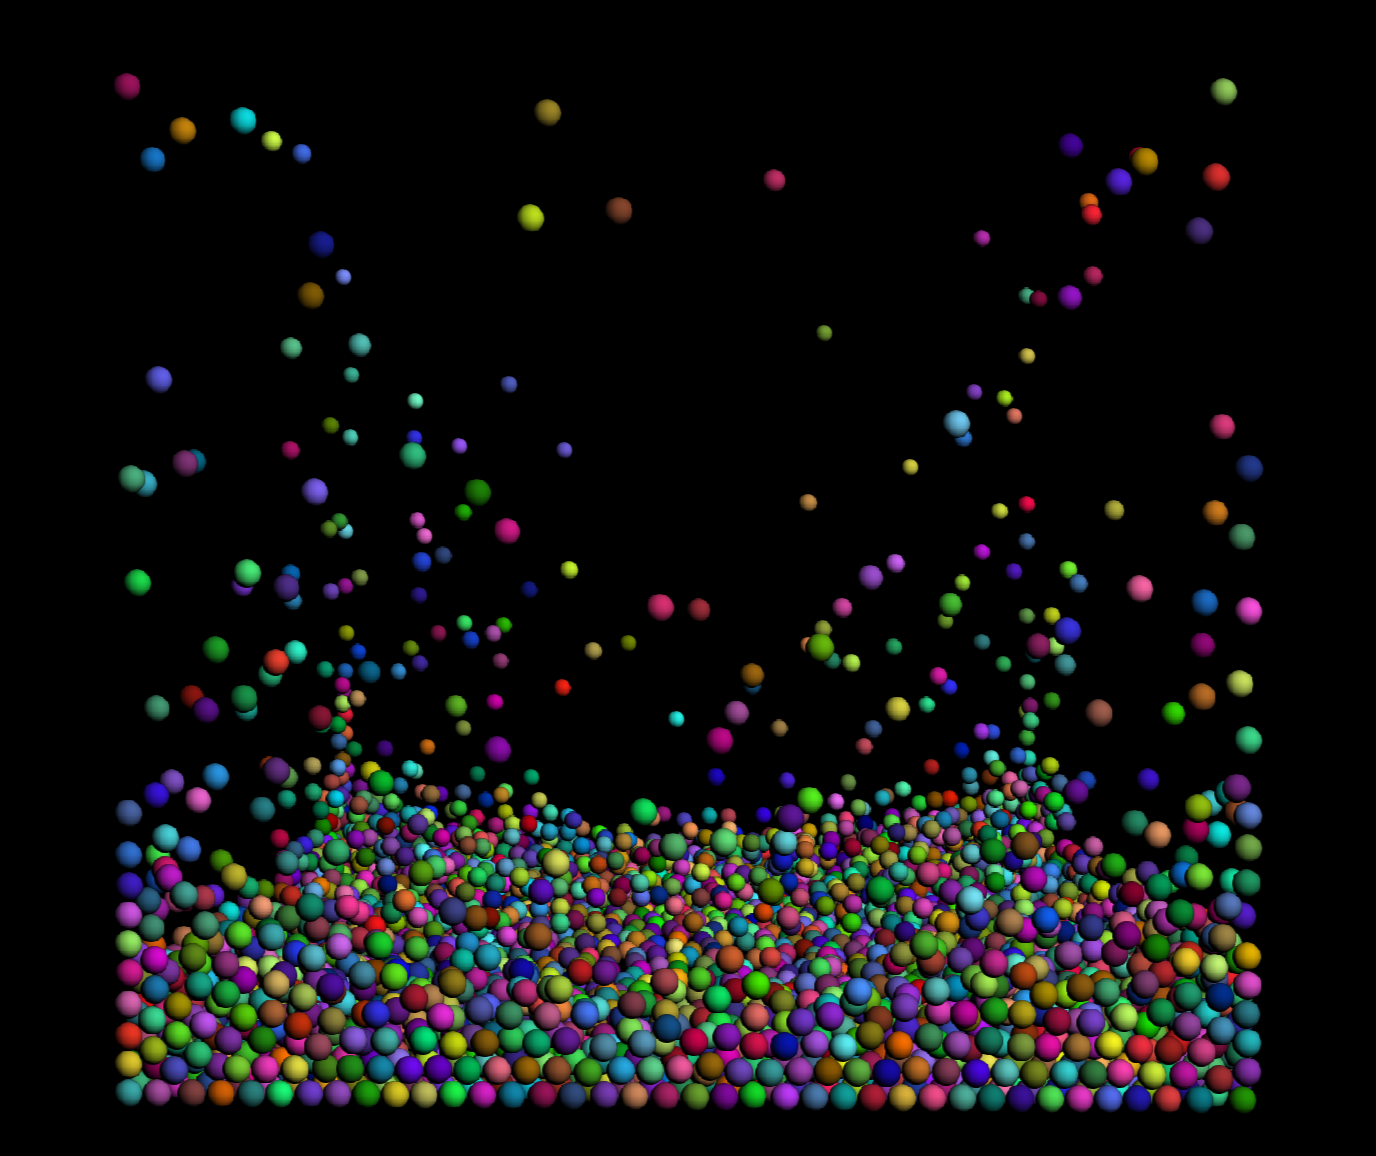
\includegraphics[scale=0.20]{figures/simulation.png}
  \captionsetup{justification=centering}
  \captionsetup{format=hang}
  \singlespace
  \caption{Simulation involving 4,096 particles. The box is invisible.}
\end{figure}

%  Starting Paragraph One
\indent\indent 
The main simulation consists of 4,096 identical particles, each having a radius of 0.4 units and a mass of 1 unit. The particles are initially arranged in a $16 \times 16 \times 16$ grid, evenly spaced within the center of a $32 \times 32 \times 32$ box. Each particle is assigned a randomized velocity ranging from 0.0 to 1.0 units per second in any direction, and the acceleration due to gravity is set at 10 units per second squared. To minimize post-collision-resolution error, the system operates at a frequency of 600 steps per second.

%___________________________________________
% Subheading 1 (remove/add as needed)
\vspace{-0.4em} % This line is added to preserve the double-spaced environment since the \section command                      adds an extra space

\section{Naive Simulation}
\indent \indent This simulation uses Gauss-Seidel position-based dynamics. 
Each simulation step involves three top level loops that iterate through each particle. Pseudocode for a single simulation step is shown below.

\begin{algorithm}
  \caption{Naive Simulation Step}\label{alg:cap}
  \begin{algorithmic}
    \For{each particle}
      \State $x_0 \gets x$
      \State $v \gets v + g \Delta t$
      \State $x \gets x + v \Delta t$
      \State Bound particle in cube
    \EndFor
    \For{$i \in$ particles}
      \For{$j \in$ particles before $i$}
        \State Resolve collision between particle $i$ and $j$
      \EndFor
    \EndFor
    \For{each particle}
      \State $v \gets \frac{x - x_0}{\Delta t}$
    \EndFor
  \end{algorithmic}
\end{algorithm}

\indent\indent The $x_0$, $x$, and $v$ represents the 
current particle's previous position, current position, and current velocity, respectively. 
$g$ represents gravity and $\Delta t$ represents the seconds per step. 
The second top-level loop resolve collisions betweeen particles
and makes the entire simulation step an $O(N^2)$ process where $N$ is the number of particles.

\section{Spatial Grid Simulation}

\begin{figure}[H]
\centering
  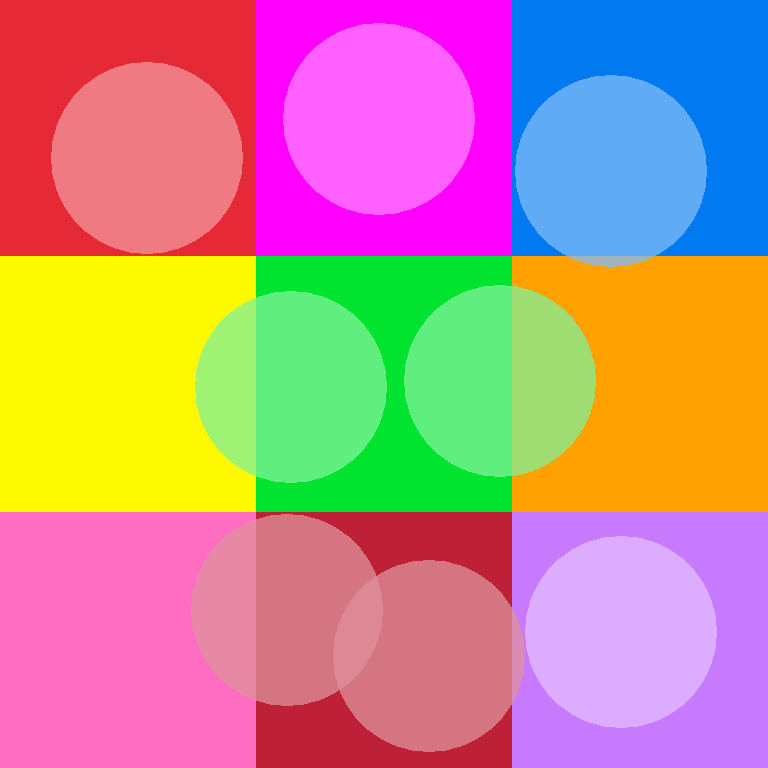
\includegraphics[scale=0.20]{figures/grid.png}
  \captionsetup{justification=centering}
  \captionsetup{format=hang}
  \singlespace
  \caption{Simulation involving 4,096 particles. The box is invisible.}
\end{figure}

\indent\indent This simulation speeds up collision detection over
the naive simulation by the usage of spatial grid, a spatial 
structure that maps the floor of the position of
each particle to the index of the particle. The spatial grid is
a three-dimensional array of linked list of indices whose dimensions
are identical to the world box. Each linked list of this grid will 
be referred to as tile for the rest of this paper. Pseudocode for a 
single simulation step is shown below.

\begin{algorithm}
  \caption{Spatial Grid Simulation Step}\label{alg:cap}
  \begin{algorithmic}
    \For{each particle}
      \State $x_0 \gets x$
      \State $v \gets v + g \Delta t$
      \State $x \gets x + v \Delta t$
      \State Bound particle in cube
    \EndFor
    \State Clear $G$
    \For{each particle}
      \State $i, j, k \gets \lfloor x \rfloor$
      \State append particle index to $G_{ijk}$
    \EndFor
    \For{$i \in$ particles}
      \For{$j \in$ particles in current and adjacent tiles}
        \State Resolve collision between particle $i$ and $j$
      \EndFor
    \EndFor
    \For{each particle}
      \State $v \gets \frac{x - x_0}{\Delta t}$
    \EndFor
  \end{algorithmic}
\end{algorithm}

\indent \indent $G$ represents the grid, and all the other
input variables are from the naive algorithm.
In the second top-level loop, the spatial grid is constructed.
In the third top-level loop, instead of looking at every
particle that comes before the current one, only the particles
in the current and adjacent tiles are looked at. 
Note, the current tile is the tile the current particle belongs to.

This is possible because each particle is smaller than a tile
and only moves a little each frame. In the average and
best case scenario $O(N)$, 
Unlike the
naive simulation, the simulation step is $O(N)$, greatly improving
performance.

\section{Edge Coloring Simulation}
This simulation speeds up collision detection ove
involves treating the grid as graph.
The tiles of the grid are treated as vertices of the graph,
and adjacent pair of tiles are treated as the edges. 
Note, that tiles are considered self-adjacent, that is an edge
is formed by tile to itself. Each tile is connected to
27 other tiles, so an edge coloring requires 27 colors.
Since the form of the graph is complile time constant,
no memory is used create the edge sets for each color. 
Instead for each step 


\vspace{-0.4em} % This line is added to preserve the double-spaced environment since the \section command                      adds an extra space

% THIS LINE ADDS THE FIRST ORDER SUBHEADING (SUBHEADING 1) TO THE TABLE OF CONTENTS (REMOVE/ADD AS NEEDED)

